\documentclass{article}
\usepackage[margin=1in]{geometry}
\usepackage{graphicx}
\usepackage{hyperref}
\title{\vspace{-2.0cm}ViReport v0.0.1}
\author{Niema Moshiri}
\date{2020-03-08}
\begin{document}
\maketitle

\section{Input Dataset}
The analysis was conducted on a dataset containing 288 sequences.
The average sequence length was 29801.0278,
with a standard deviation of 331.0522.
The earliest sample date was 2013-07-24,
the median sample date was 2020-01-29,
and the most recent sample date was 2020-03-04.


\begin{figure}[h]
\centering
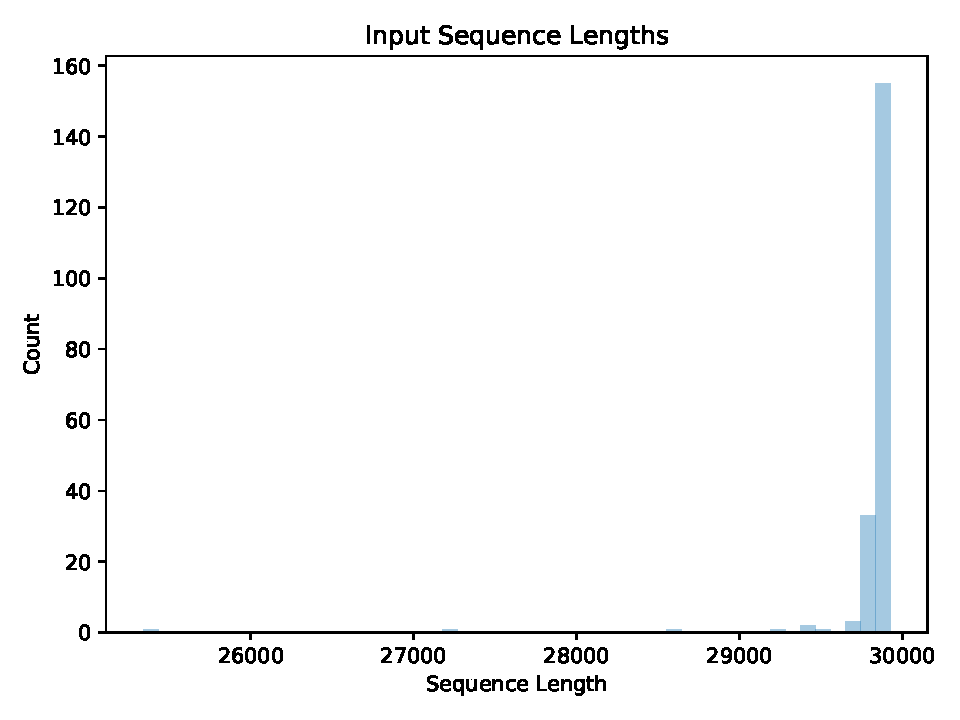
\includegraphics[width=0.75\textwidth,keepaspectratio]{./figs/input_sequence_lengths.pdf}
\caption{Distribution of input sequence lengths}
\end{figure}



\begin{figure}[h]
\centering
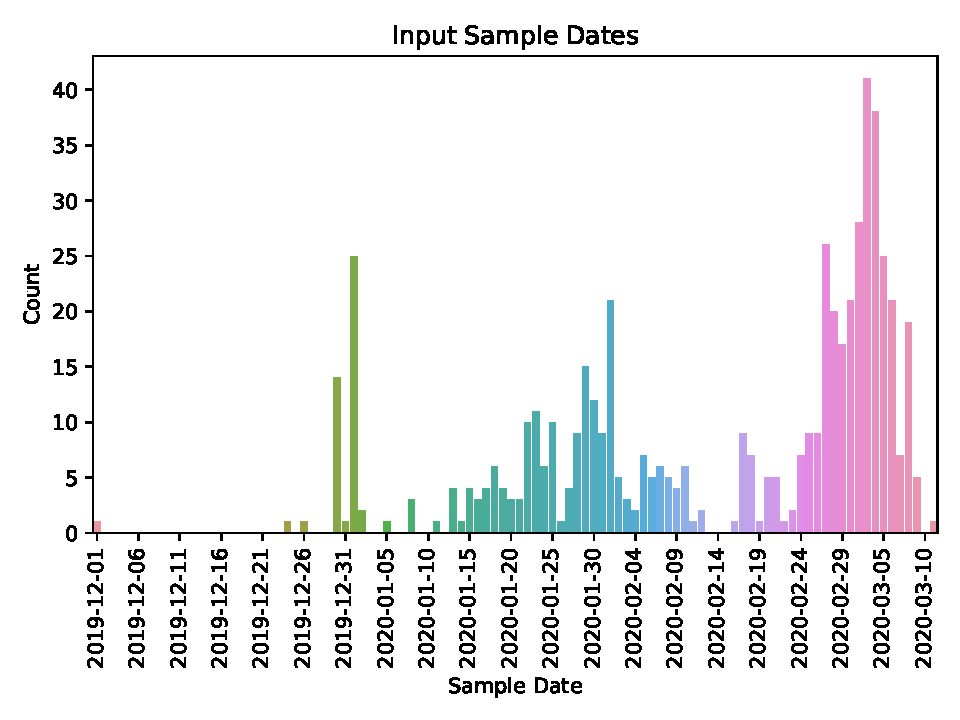
\includegraphics[width=0.75\textwidth,keepaspectratio]{./figs/input_sample_dates.pdf}
\caption{Distribution of input sample dates}
\end{figure}

\section{Preprocessed Dataset}
The input dataset was preprocessed such that sequences were given safe names: non-letters/digits in sequence IDs were converted to underscores.
After preprocessing, the dataset contained 288 sequences.
The average sequence length was 29801.0278,
with a standard deviation of 331.0522.
The earliest sample date was 2013-07-24,
the median sample date was 2020-01-29,
and the most recent sample date was 2020-03-04.


\begin{figure}[h]
\centering
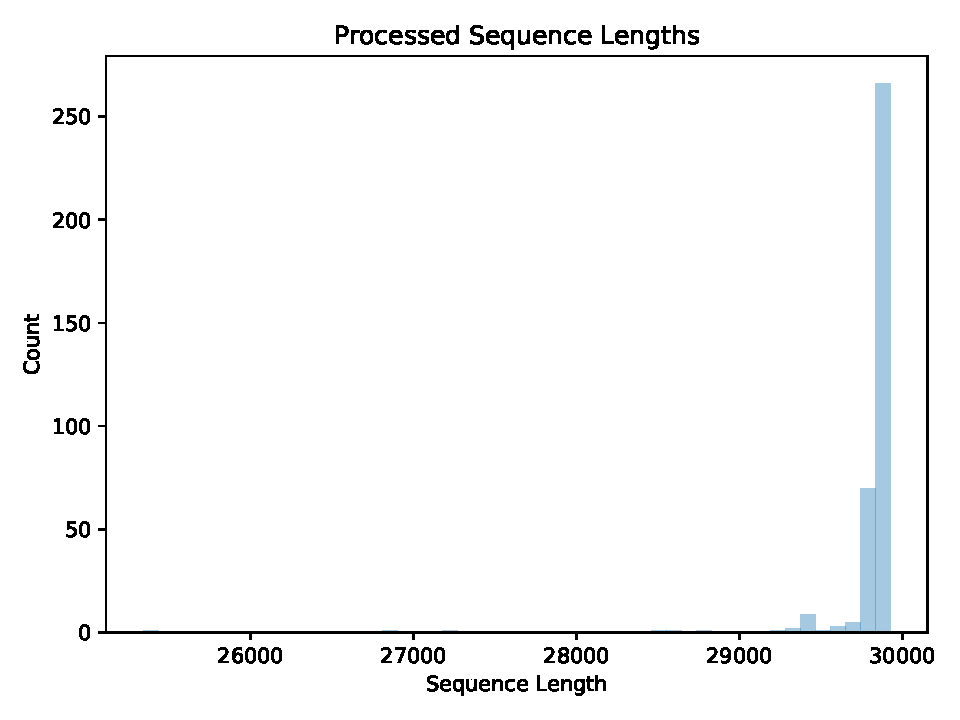
\includegraphics[width=0.75\textwidth,keepaspectratio]{./figs/processed_sequence_lengths.pdf}
\caption{Distribution of preprocessed sequence lengths}
\end{figure}



\begin{figure}[h]
\centering
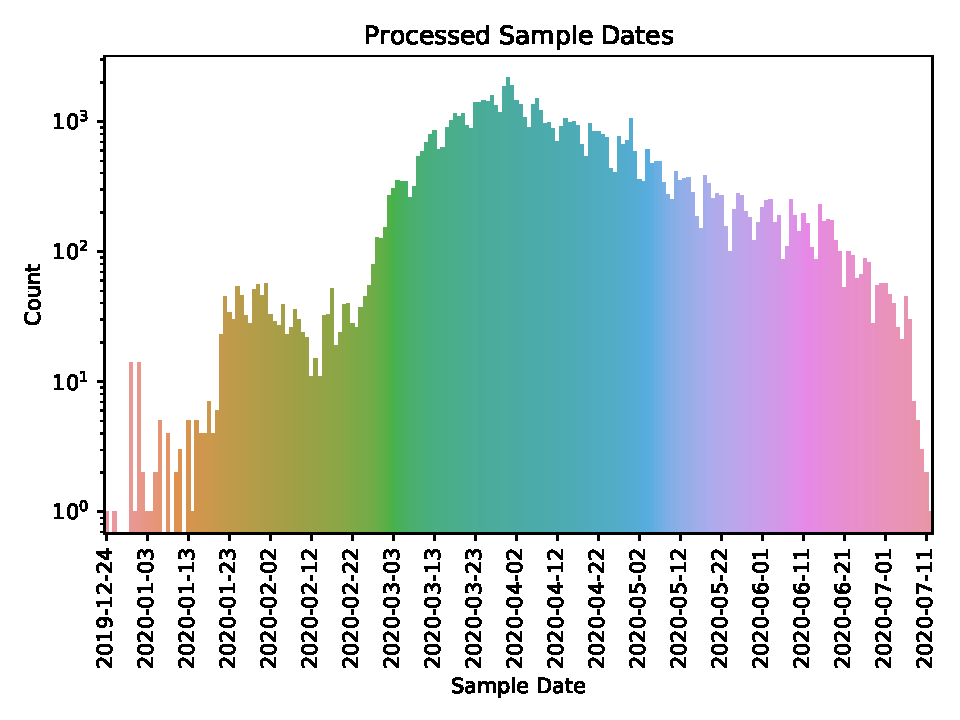
\includegraphics[width=0.75\textwidth,keepaspectratio]{./figs/processed_sample_dates.pdf}
\caption{Distribution of preprocessed sample dates}
\end{figure}

\section{Multiple Sequence Alignment}
Multiple sequence alignment was performed using MAFFT (Katoh \& Standley, 2013) in automatic mode.
There were 30205 positions (15195 invariant) and 251 unique sequences in the multiple sequence alignment.
Pairwise distances were computed from the multiple sequence alignment using the tn93 tool of HIV-TRACE (Pond et al., 2018).
The average pairwise sequence distance was 0.000257,
with a standard deviation of 0.000215.


\begin{figure}[h]
\centering
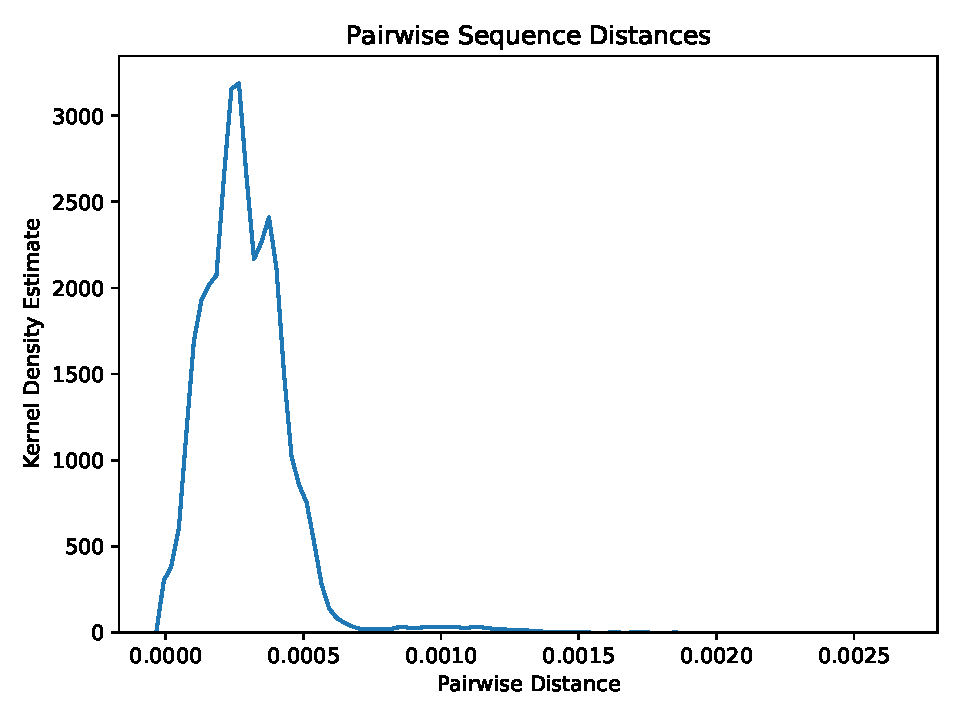
\includegraphics[width=0.75\textwidth,keepaspectratio]{./figs/pairwise_distances_sequences.pdf}
\caption{Distribution of pairwise sequence distances}
\end{figure}

\section{Phylogenetic Inference}
A maximum-likelihood phylogeny was inferred using IQ-TREE (Nguyen et al., 2015) in ModelFinder Plus mode (Kalyaanamoorthy et al., 2017).
The inferred phylogeny was MinVar-rooted using FastRoot (Mai et al., 2017).
Pairwise distances were computed from the phylogeny using TreeSwift (Moshiri, 2020).
The maximum pairwise phylogenetic distance (i.e., tree diameter) was 0.00323,
and the average pairwise phylogenetic distance was 0.000407,
with a standard deviation of 0.000329.


\begin{figure}[h]
\centering

\includegraphics[width=1\textwidth,height=1\textheight,keepaspectratio]{./figs/tree_mutations.pdf}
\caption{Rooted phylogenetic tree in unit of expected per-site mutations}
\end{figure}



\begin{figure}[h]
\centering
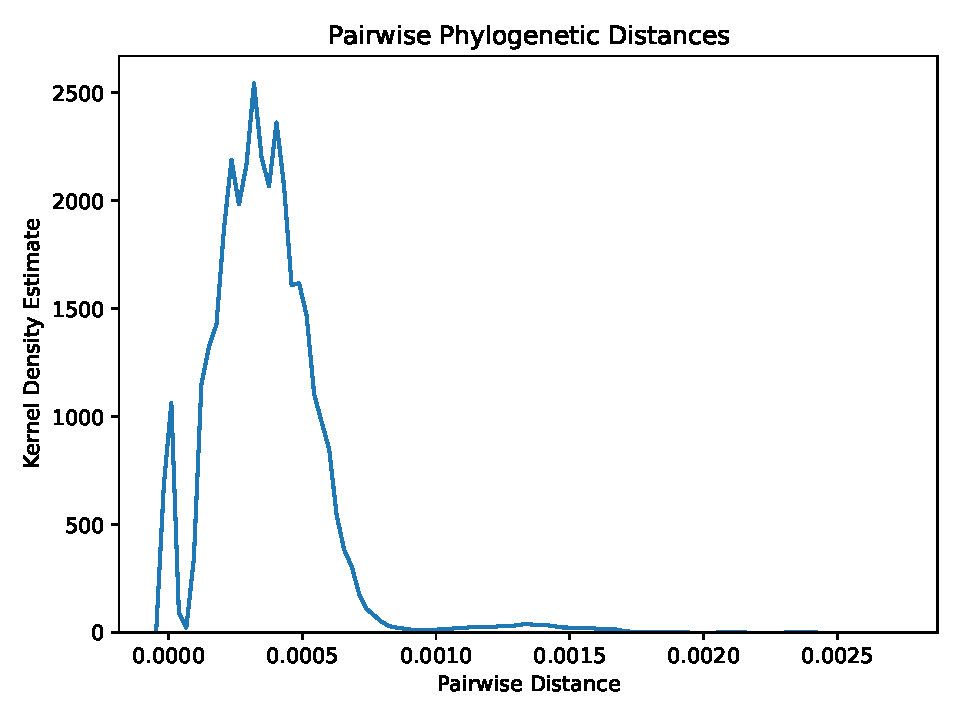
\includegraphics[width=0.75\textwidth,keepaspectratio]{./figs/pairwise_distances_tree.pdf}
\caption{Distribution of pairwise phylogenetic distances}
\end{figure}

\section{Phylogenetic Dating}
The rooted phylogeny was dated using treedater (Volz \& Frost, 2017).
The height of the dated tree was 0.406 days,
so given that the most recent sample was collected on 2020-03-04,
the estimated time of the most recent common ancestor (tMRCA) was 2020-03-03.


\begin{figure}[h]
\centering
\includegraphics[width=1\textwidth,height=1\textheight,keepaspectratio]{./figs/tree_time.pdf}
\caption{Dated phylogenetic tree in unit of years}
\end{figure}

\section{Transmission Clustering}
Transmission clustering was performed using TreeN93 (Moshiri, 2018) using pairwise phylogenetic distances.
The total number of singletons (i.e., non-clustered individuals) was 47,
and the total number of clusters (excluding singletons) was 14.
The average cluster size (excluding singletons) was 16.5,
with a standard deviation of 31.771,
and the maximum and minimum cluster sizes were 125 and 2, respectively.


\begin{figure}[h]
\centering
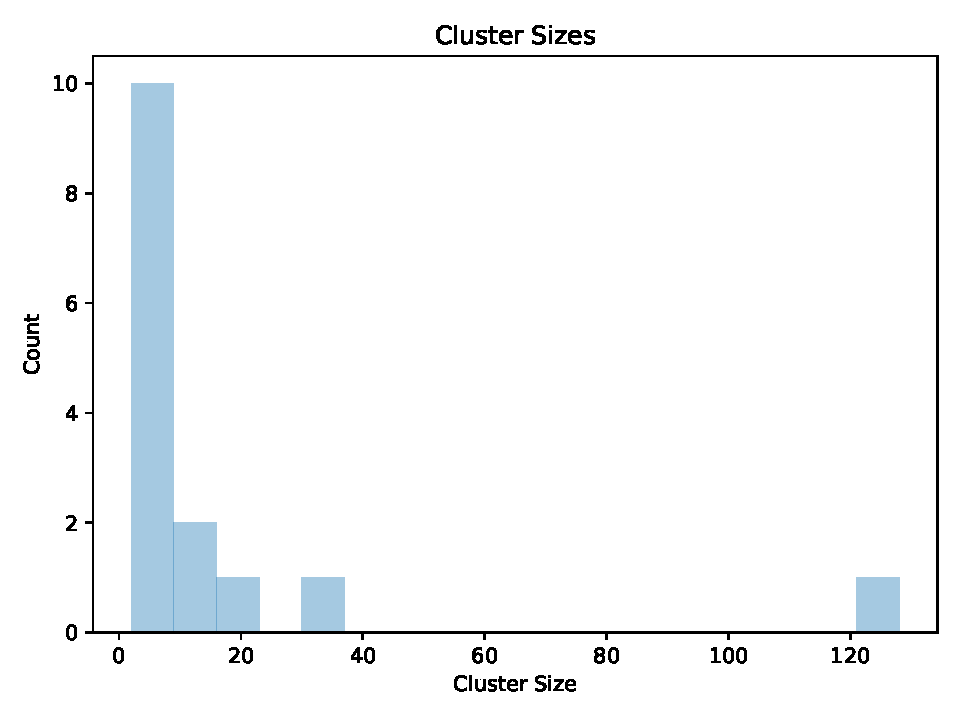
\includegraphics[width=0.75\textwidth,keepaspectratio]{./figs/cluster_sizes.pdf}
\caption{Distribution of cluster sizes (excluding singletons)}
\end{figure}


\end{document}
